\documentclass[12pt]{article}
%\usepackage{apacite}
\usepackage{wrapfig}
\setlength{\parindent}{0pt}
\usepackage{tgtermes}
\usepackage{setspace}
\usepackage{gensymb}
\doublespacing
\usepackage{graphicx}
\usepackage{float}
\usepackage[utf8]{inputenc}
\usepackage[backend=biber,style=apa,autocite=inline]{biblatex}
\usepackage{fancyhdr}
\pagestyle{fancy}
\lhead{Paper 1}
\rhead{Victor M. Poulsen, Studie Nr.: 201707639}

\DeclareLanguageMapping{english}{english-apa}
\addbibresource{References.bib}
\setcounter{page}{1}

\title{Affective modulation of weighting function}
\author{Victor Møller Poulsen, Studie Nr.: 201707639}

\begin{document}
\maketitle
\leavevmode

\section{Description}
Both Expected-utility theory and prospect theory
posit that humans maximize some version of
utility. The theories get there by a
combination of two functions
\autocite{rottenstreich2001money}.
A value function $v$ transforms objective value to
subjective utility, and a weighting function $w$
distorts probabilities \autocite{rottenstreich2001money,
gonzalez1999shape}. Expected-utility and
prospect theory combine these two paramters in
the simplest way possible
\autocite{rottenstreich2001money}

\[
	\sum w(p_i)v(i),
\]

where $p$ stands for probability and $i$ stands for the
$i^{th}$ gamble.

Prospect Theory \autocite{PT,
tversky1992advances} (PT) is arguably the main model
of human decision making \autocite{
newell2015straight}. It advances theorizing
from expected-utility by postulating that losses and
gains are evaluated as changes in wealth rather
than in regard to end states \autocite{newell2015straight}.

\vspace{3mm}

In \textcite{PT} we find the familiar
(non-linear) S-shaped
value function $v$ which is concave for the gains
domain and convex for losses (where it is steeper as well).
The weight function $w$ is the identity,
$w(p) = p$ in expected-utility theory
\autocite{rottenstreich2001money} whereas
a non-linear probability distortion is proposed in
prospect theory \autocite{PT}. Here $w$
is stylized as being reverse S-shaped,
meaning that it is concave for low probabilities
and convex for high probabilities \textcite{
gonzalez1999shape}. This means that
people underweight changes in probability in
the middle of the spectrum (e.g. $[0.2-0.8]$)
while overweighting changes in probability close
to the end-points (e.g. $[0.0 - 0.2], [0.8 - 1.0]$).
These general characteristics of the weighting
function are empirically well documented
\autocite{tversky1992advances,
wu1996curvature}.

\subsection{Prior work}

There is evidence to support
the notion that the affect of outcomes modulates
the parameters of both $v$
\autocite{hsee2004music} and $w$ \autocite{
rottenstreich2001money}. A main finding is
that the S-shape of the weighting function
$w$ appears to be more pronounced
for high-affect than low-affect outcomes under
uncertainty \autocite{rottenstreich2001money}.
This was shown as a preference reversal in
which a high-affect outcome was preferred for
low probability (1\%) whereas a low-affect
outcome was preferred for high probability (100\%)
\autocite{rottenstreich2001money}.
The finding that affect appears to modulate
both $v$ and $w$ has subsequently been
modelled as an interaction between an
affective system and a deliberative system \textcite{
	mukherjee2010dual,
mukherjee2011thinking}.

\subsection{Focus and parameterization}

In this article we focus exclusively on the
weighting function $w$ while ignoring both
the value function $v$ and the combination
of the two functions. We also restrict ourselves
to the gains domain.
In \textcite{rottenstreich2001money} they
propose that the affective modulation can
be estimated as an affect paramter $a$
in the form:

\[
	w(p) = \frac{p^{1-a}}
	{p^{1-a}+(1-p)^{1-a}}
.\]

where $a \in [0, 1]$ and larger values indicate
greater affect
and more curvature \autocite{rottenstreich2001money}.
The issue with this one-parameter
formulation is that it
does not account for the fact that people
generally show low \emph{elevation}.
What I mean by that is that the empirically
observed weighting function $w$ typically
crosses the diagonal line
at around $0.3$ rather than $0.5$
\autocite{gonzalez1999shape}. The one-parameter
formulation fixes this point at $0.5$
which can be seen from figure $1$.

\begin{figure}[h!]
	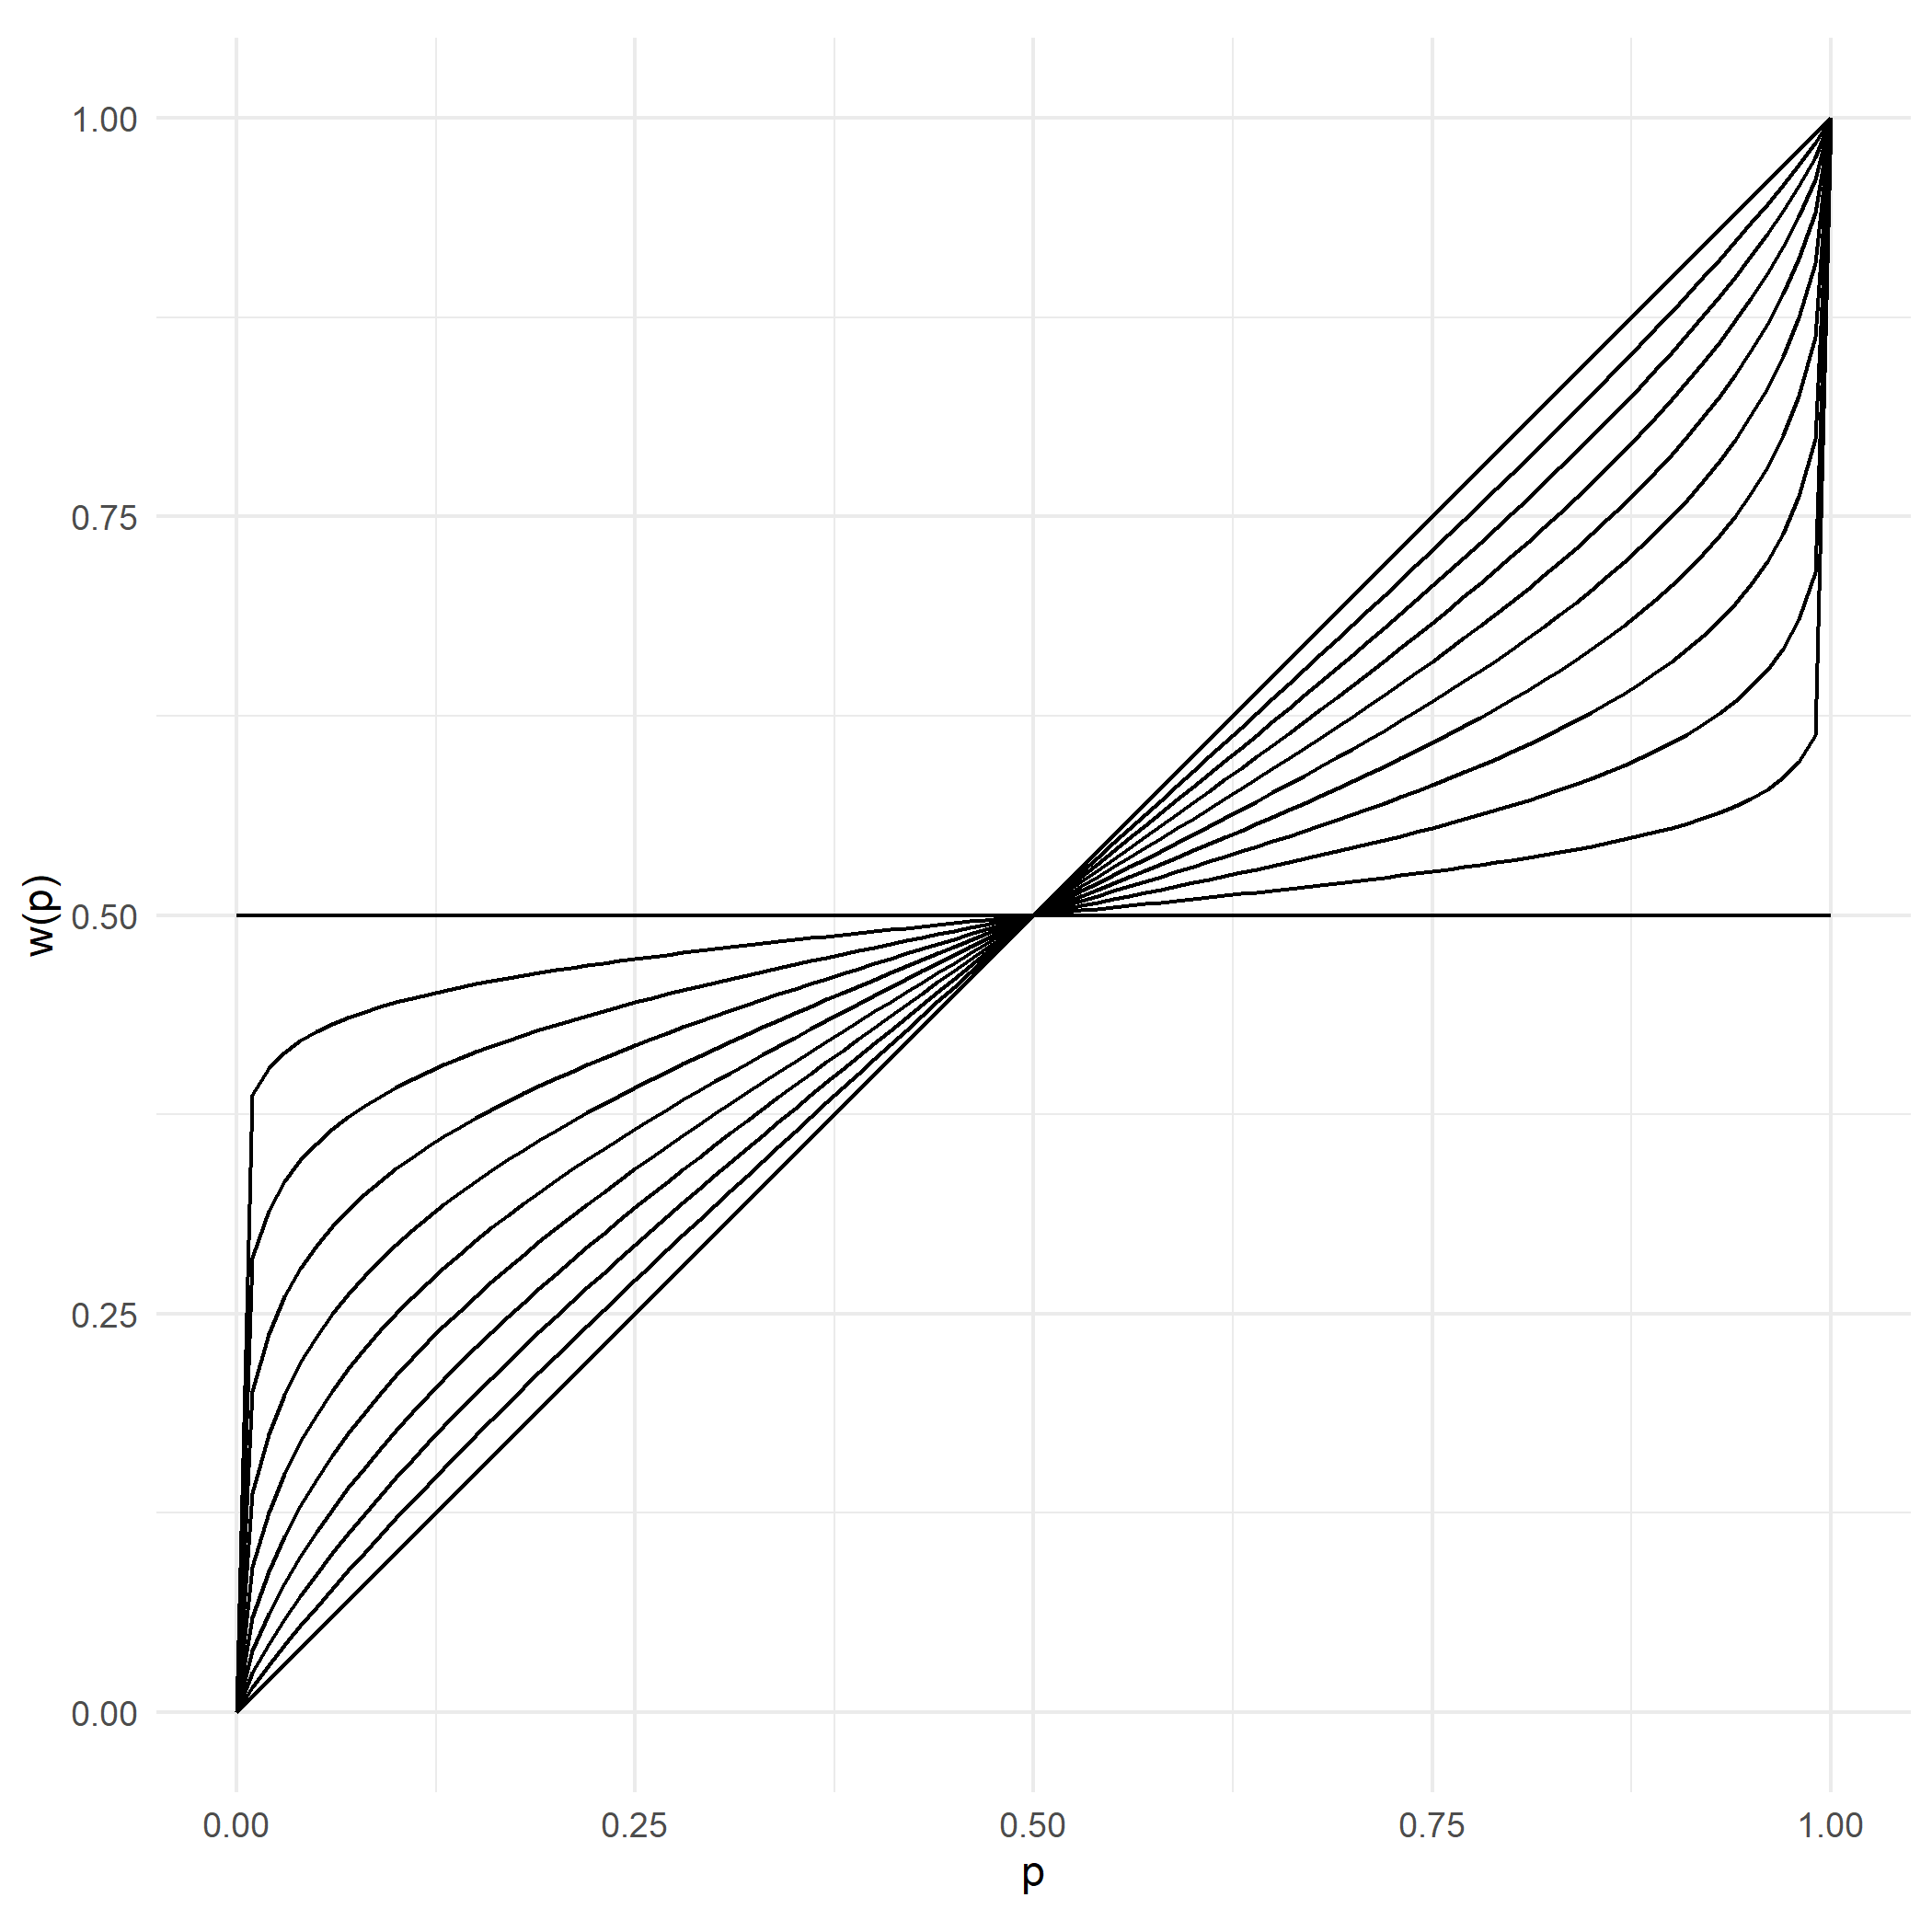
\includegraphics[width = \linewidth]{../Figures/oneParam.png}
	\caption{Data simulated from the model
		$w(p) = \frac{p^{1-a}}
		{p^{1-a}+(1-p)^{1-a}}$ with
		$a \in [0, 1]$. Diagonal line has
		$a = 0$, and the horizontal line
		has $a = 1$. Intermediate curves
		are generated for $0.2$ increments
		of $a$. All values beside
		$a = 0$ show a probability distortion
		as compared to the objective probability.
		Note that all curves meet at
		$w(p) = 0.5, p = 0.5$. This is
	not empirically supported.}
\end{figure}

Instead of using the parameterization
proposed in \textcite{rottenstreich2001money}
this paper will use the parameterization
of $w$ proposed in \textcite{gonzalez1999shape}.
They parameterize $w$ with two parametrs;
$\delta$ and $\gamma$.

\vspace{3mm}

The $\delta$ parameter will vary based on
\emph{elevation} (intercept)
\autocite{gonzalez1999shape},
which here simply refers to the overall
perceived attractiveness of outcomes
under uncertainty.

\vspace{3mm}

The $\gamma$ parameter will vary based on
\emph{curvature} (slope)
\autocite{gonzalez1999shape} and is what we
are primarily interested in for our purposes.
It follows as a direct prediction from
\textcite{rottenstreich2001money} that the
curvature ($\gamma$) should be modulated by changes in
the affective level of outcomes. See
figure 2 for an illustration of how the $\delta$
and $\gamma$ parameters independently modulate
different aspects of the weighting function $w$.

\begin{figure}[h!]
	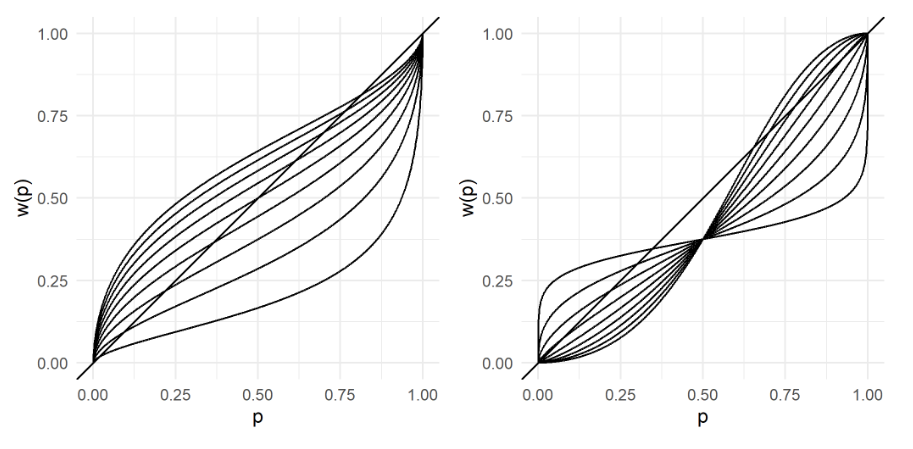
\includegraphics[width = \linewidth]{../Figures/Fig2.png}
	\caption{Data simulated from the model
		$w(p) = \frac{\delta \cdot p^{\gamma}}
	{\delta \cdot p^{\gamma} +
	(1-p)^{\gamma}}$ similarly to figure 4
	of \textcite{gonzalez1999shape}.
	On the left: $\gamma$ fixed at $0.6$
	and $\delta$ varied between $0.2$ and $1.8$.
	On the right: $\delta$ fixed at $0.6$
	and $\gamma$ varied between $0.2$ and $1.8$.
	Shows that $\gamma$  controls
	curvature and $\delta$ controls
	elevation. The identity function $w(p) = p$
	is achieved for $\delta = 1, \gamma = 1$.
	Note.. gamma low has the opposite interpretation
	as compared to rottenstreich?}
\end{figure}



\vspace{3mm}

The model is:

\[
	\log\frac{w(p)}{1-w(p)} =
	\gamma \log\frac{p}{1-p} + \tau
.\]

where solving for $w(p)$ and setting $\delta = \exp(\tau)$
gives us

\[
	w(p) = \frac{\delta \cdot p^{\gamma}}
	{\delta \cdot p^{\gamma} +
	(1-p)^{\gamma}}
.\]

The above equations are taken from \textcite{
rottenstreich2001money}.

\subsection{Methodology}

Two studies are proposed to
properly test the robustness
of affect-level on the
curvature ($\gamma$) of the
weight function $w$.

\vspace{3mm}

In the first study, subjects will be asked to
rate the affect-richness of 10 different
items.
All outcomes
consist of coupons redeemable
for various items, all worth $\$500$.
The 10 items are designed to cover the
full spectrum from affect-rich to
affect-poor.

\vspace{3mm}

Example of expected high-affect item:\\
"If you won a $\$500$ coupon redeemable
for a vacation abroad how emotionally
affected would you be?"

\vspace{3mm}

Example of expected low-affect item: \\
"If you won a $\$500$ coupon redeemable
for insurance covering how emotionally
affected would you be?"

\vspace{3mm}

For the full list of items see Appendix $A$.
Participants
will indicate how affect-rich
each outcome is with a slider. Participants will
see "not affected at all" (left),
"somewhat affected" (middle)
and "very affected" (right).
We will receive continuous ratings from $0$
(affect poor) to $1$ (affect rich). A mean
affect rating across participants for each
item will rank them from least affective to
most affective. Three items (gambles) are
then selected: The least affective item,
the most affective item and the item in
between these two extremes which separate them
best (follow up).

\vspace{3mm}

In the second study, subjects will be presented
with the three items which have been validated
for affect-richness in the prior study.
In this study however, the formulation
around the items is that of a gamble.
The formulation is the same
for all items: \\

"You can buy a lottery ticket with an $[x]$
percent chance of winning a $\$500$ coupon
redeemable for $[y]$ with a $[1-x]$ percent
chance of winning nothing. How much are you
willing to pay for the lottery ticket?" \\

The three selected items are inserted as $[y]$
and $100$ different probability levels:
$x = 0.01, 0.02, \ldots, 0.99$ will be
inserted as $[x]$ and the negation $[1-x]$.
With all
possible combinations, this means that
all participants will rate $3$ items
at $100$ different levels of certainty each.
As in experiment 1 participants will rate
with a slider. This time ranging from
$\$0$ to $\$500$ as it is neither logical
to assign a value below $\$0$ or above
$\$500$ to any of the gambles.
The approach is somewhat
different from \textcite{gonzalez1999shape}
but ultimately we estimate the same thing that
they do; participants' certainty equivalence (CE).
This simply is the amount of money they think
that the gamble is worth. \\

Note that we are not directly measuring either
$\delta$ or $\gamma$. What we do measure is the
dependent variable $w(p)$ and the independent
variable $p$ for items ranked based on their
affect-richness. \\

In order to infer the
unmeasured paramters a bayesian (non)linear
mixed effects model is proposed. The model
is fitted in $R$ with the  $brms$ package.
Here we can specify the previously
mentioned formula:

 \[
	 w(p) \sim \frac{\exp({\tau})\cdot p^{\gamma}}
	 {\exp({\tau})\cdot p^{\gamma}+(1-p)^{\gamma}}
.\]

We have to specify that the model should
be nonlinear. We can further specify that we would like to
estimate specifically the value for $\tau$
and $\gamma$ with random intercepts (partial pooling)
for participants (ID) and with item as a main
effect. \\

 \[
	 \tau \sim 0 + item + (1|ID),
\]
\[
	\gamma \sim 0 + item + (1|ID)
.\]

We can then convert $\tau$ to $\delta$
by exponentiating the estimated value
for $\tau$ for each item. For the analysis
pipeline on simulated data, see Github. \\

After fitting the model, posterior samples
for the three items are generated. Based on
these, $.66$ and $.95$ credibility intervals
are calculated and the distributions for each
paramter (for each item) as a group-level effect
is visualized. \\

\emph{Hypothesis:} A directional effect is
expected for the population effect of the
$\gamma$ parameter. It is expected that
item 1 (lowest affect) will have the highest
$\gamma$ value, and that item 3 (highest affect)
will have the lowest $\gamma$ value, with
item 2 falling in the middle. The paper
does not propose to calculate significance
or bayes factor, but simply hypothesizes that
the $.95$ and $.66$ credibility intervals
will only overlap in the expected direction
(see plot).







but a thorough investigation
of this effect is lacking. This study consits
of two sub-studies. In the first study subjects
will evaluate 10 items on a scale of affect.
In the second study subjects will indicate their
certainty equivalence (CE) as to gambles
involving these questions. Based on this, the
parameters of the weighting function

\[
	w(p) = \frac{\delta \cdot p^{\gamma}}
	{\delta \cdot p^{\gamma} + (1-p)^{\gamma}}
\]

are estimated for each of the 10 items, and it
is calculated whether level of affect (obtained in
study 1) modulates the parameters of the weighting
function. Note that the above is the two-parameter
weighting function
suggested in \autocite{gonzalez1999shape}.

\section{Hypotheses}

$H_1$: It is expected that the 10 questions in
study 1 will - on average - obtain significantly
different ratings as to affective quality.
This is necessary for the follow-up study to
make sense.

$H_2$ It is hypothesized that the $\gamma$
parameter will be higher for items that are
rated as being higher in affect.
(estimate of size of effect).

$H_3$: It is expected that the $\delta$
parameter will not be systematically
modulated by the level of affect of items.

\section{Design Plan}

\textbf{Study type:} Observational Study. \\

\textbf{Blinding:} No blinding is involved in this study. \\

\subsection{Study Design}

\emph{Study 1}: All subjects will rate all items
(see Appendix 1) as to the level of affect they
feel with regards to them.

\emph{Study 2}: All participants
indicate their certainty equivalence (CE) for all
combinations of items (10) and certainty levels
(1\%, 5\%, 15\%, 30\%, 50\%, 70\%, 85\%, 95\%, 99\%).
This results in $90$ observations per participant.

\section{Sampling Plan}

\textbf{Existing Data}: Registration prior
to creation of data.

\textbf{Data collection procedures}:
Participants will be recruited through online
channels (e.g. facebook, student groups, etc.).
Participants must be at least 18 years old to
participate. In the first experiments subjects
will be payed 30 DKK for agreeing to participate
in an approx. 10 minute online survey. In the
second experiment subjects will be payed 150 DKK
for agreeing to participate in an approx. 60 minute
online survey.

\textbf{Sample size}:

\emph{Study 1}: 30 participants. \\
\emph{Study 2}: 50 participants.

\textbf{Sample size rationale}:

Power analysis?
Credibility/Density interval 95\%
assuming data generating process?

\section{Variables}

\subsection{Manipulated variables}
\emph{Study 1}: No manipulated variables. \\

\emph{Study 2}: Levels of uncertainty are
manipulated, and are given as
$0.01, 0.05, 0.15, 0.3, 0.5, 0.7, 0.85, 0.95, 0.99$.
Levels of affect differ for each item
(obtained in Study 1).

\subsection{Measured variables}
\emph{Study 1}: The single outcome variable
will be the rating of affect level. This will
be measured on a scale of $0-100$ using a
slider.

\emph{Study 2}: The single outcome variable
is the price that subjects indicate that they
are willing to pay for a ticket in a lottery
(combination of probability of outcome).
This will indicate their certainty equivalence (CE).
This will be measured on a scale of $0-500$ dollars
using a slider. The max is 500 dollars since the
lottery tickets by definition cannot be worth
more than this (see Appendix 2).

\subsection{Indices}

??

\section{Analysis Plan}

All analysis is performed in the programming
language $R$ \autocite{rcore} using $Rstudio$
\autocite{rstudio}. \\

\emph{Study 1}: The affect ratings will be
ordered based on group-level means? \\

\emph{Study 2}: A bayesian generalized nonlinear
mixed effects model is fit to the data using the
$R$ package $brms$ \autocite{brms}.
This is done to estimate the unobserved parameters
$\delta$ and $\gamma$ from the independent variable
probability/uncertainty and the dependent variable
$w(p)$ which is the observed certainty equivalence (CE).
Weakly informative priors are specified for both
$\gamma$ and $\delta$ (see Github).


\section{Discussion}

\printbibliography
\end{document}


